\documentclass[a4paper, 12pt]{article}

\usepackage{tikz}
\usetikzlibrary{positioning}
\usetikzlibrary{chains}
\usetikzlibrary{arrows.meta}

\title{Task 3}
\author{}
\date{}

\begin{document}
\maketitle

\begin{figure}[h]
  \centering
  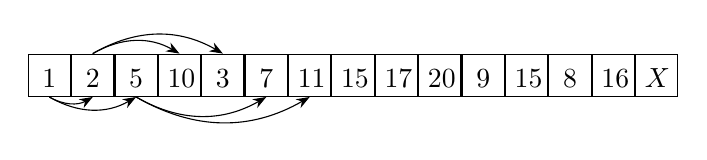
\begin{tikzpicture}[
    start chain,
    node distance=0,
    auto,
    every node/.style={
      rectangle,
      text width=2ex,
      text height=2ex,
      align=center,
      draw
    },
    >=Stealth,
    ]

    \foreach \x/\y in {1/1,2/2,5/3,10/4,3/5,7/6,11/7,15/8,17/9,20/10,9/11,15/12,8/13,16/14,X/15}{
      \node (\y) [on chain] {$\x$};
    }

    \path[->]
    (1.south) edge[bend right] (2.south)
    (1.south) edge[bend right] (3.south)
    (3.south) edge[bend right] (6.south)
    (3.south) edge[bend right] (7.south)
    (2.north) edge[bend left]  (4.north)
    (2.north) edge[bend left]  (5.north)
    ;
  \end{tikzpicture}
\end{figure}


\end{document}
